\documentclass[12pt,a4paper]{report}
\usepackage{graphicx}
\usepackage{tikz}
\usepackage{multicol}
\usepackage{blindtext}
\usepackage{xpatch}
\usepackage{mathptmx}
\usepackage{amssymb}
\usepackage{float}
\usepackage{geometry}
\usepackage{algorithm}
\usepackage{algpseudocode}
\usepackage{multirow}
\geometry{
    right=25mm,
    left=25mm,
    top=25mm,
    bottom=25mm
}
\graphicspath{{images/}}



% Begin document
\begin{document}

% Cover
\pagenumbering{gobble}
\begin{center}
\vspace{4cm}

{\Huge\textbf{QUADRUPED ROBOT}}\\
\vspace{2cm}

\Large PROJECT REPORT\\
\vspace{1.75cm}

Submitted by\\
\vspace{0.5cm}
\large Abdul Ahad\\
\large Atul Vyshnav R\\
\large Krishnanand K\\ 
\large Shinas Shaji\\
\vspace{1.5cm}

Under the supervision of\\
\large Dr. Sunil Kumar\\
\vspace{1.5cm}


\includegraphics[width=0.45\textwidth]{logoRIT}

\vspace*{\fill}
\end{center}

\begin{center}
    \large Department of Electrical and Electronics Engineering\\
\large Govt. Rajiv Gandhi Institute of Technology, Kottayam\\
\large Velloor, Pampady, Kottayam - 686501\\
\end{center}

% Declaration
\newpage
\pagenumbering{roman}
\begin{center}
\addcontentsline{toc}{chapter}{Candidate's Declaration}
%\vspace{1.5cm}

\begin{center}   

\includegraphics[width=0.35\textwidth]{logoRIT}
\end{center}
\vspace{0.5cm}
    \large Department of Electrical and Electronics Engineering\\
\large Govt. Rajiv Gandhi Institute of Technology, Kottayam\\
\large Velloor, Pampady, Kottayam - 686501\\
\vspace{2 cm}

\textbf{\underline{CANDIDATE'S DECLARATION}}\\
\vspace{0.5cm}
\end{center}

We, Abdul Ahad (Reg No: KTE18EE002), Atul Vyshnav R (Reg No: KTE18EE022), Krishnanand K (Reg No: KTE18EE040) \& Shinas Shaji (Reg No: KTE18EE053) students of B.Tech at APJ Abdul Kalam Technological University, hereby declare that the Project Dissertation titled "Quadruped Robot", which is submitted by us to the Department of Electrical and Electronics Engineering, Govt. Rajiv Gandhi Institute of Technology, Kottayam, in fulfillment of the requirement for awarding of the Bachelor of Technology degree, is not copied from any source without proper citation. This work has not previously formed the basis for the award of any Degree, Diploma, Fellowship or other similar title or recognition.

% \begin{description}
%   \item [Title of the Paper] Identification of IUU Transshipment Activity Using AIS Data.
%   \item[Author names] Harshit Muhal, Ishan Chaudhary, Kirti Dabas 
%   \item[Name of Conference/Journal] International Conference for Emerging Technology 2022
%   \item [Conference Dates with the venue (if applicable)]Online (27-29 May 2022)
%   \item [Have you registered for the conference (Yes/No)?] Yes
%   \item [Status of paper (Accepted/Published/Communicated)] Accepted
%   \item [Date of paper acceptance] 02 FEBRUARY 2022
%   \item [Date of paper publication] YET TO BE PUBLISHED
% \end{description}

% \begin{minipage}{4cm}
% \begin{flushleft}
% \vspace{5 cm}
                         
% Place: Pamapdy\\
% Date: 11/05/2022\\

% \end{flushleft}
% \end{minipage}

% \begin{minipage}{16.5cm}
% \centering
% \begin{flushleft}                                      
% \vspace{5 cm}

% Was this what you were trying, or did you have something else in mind?
% Try to add the date as well. Preferably below the names👍
% Shouldn't there be space above the names for us to sign? Are they there or am I not seeing them??
% Isnt there plennnnty of space?
% Compiling...Alright🫡

\vspace*{\fill}

\begin{multicols}{4}
\centering

\textbf{Abdul Ahad}
\vspace{0.2cm}
\textbf{(KTE18EE002)}\\
\vspace{0.2cm}

\textbf{Atul Vyshnav R}
\vspace{0.2cm}
\textbf{(KTE18EE022)}\\
\vspace{0.2cm}

\textbf{Krishnanand K}
\vspace{0.2cm}
\textbf{(KTE18EE040)}\\
\vspace{0.2cm}

\textbf{Shinas Shaji}
\vspace{0.2cm}
\textbf{(KTE18EE053)}\\
\vspace{0.2cm}

\end{multicols}

\vspace{1cm}
\begin{multicols}{2}

\flushleft Date: xxth of June, 2022

\flushright Place: Pampady, Kottayam, Kerala

\end{multicols}

% \end{flushleft} 
% \end{minipage}

% Certificate
\newpage
\begin{center}
    \begin{center}   
        
\includegraphics[width=0.35\textwidth]{logoRIT}
    \end{center}
\vspace{0.5cm}
    \large Department of Electrical and Electronics Engineering\\
\large Govt. Rajiv Gandhi Institute of Technology, Kottayam\\
\large Velloor, Pampady, Kottayam - 686501\\
\vspace{2 cm}

\textbf{\underline{CERTIFICATE}}\\
\vspace{0.5cm}
\end{center}

This is to certify that this report titled "Quadruped Robot" submitted by Mr. Abdul Ahad (Reg No: KTE18EE002), Mr. Atul Vyshnav R (Reg No: KTE18EE022), Mr. Krishnanand K (Reg No: KTE18EE040) and Mr. Shinas Shaji (Reg No: KTE18EE053) to APJ Abdul Kalam Technological University in partial fulfillment of the requirements for the award of Degree of Bachelor of Technology in Electrical and Electronics Engineering, is a bonafide record of the project carried out by them under our guidance and supervision. This report in any form has not been submitted to any other University or Institute for any purpose. 


% Abstract
\newpage
\begin{center}
\addcontentsline{toc}{chapter}{Abstract}
\Large \textbf{ABSTRACT}\\
\end{center}
\vspace{0.5cm} 

\textit{Keywords: Quadruped, Autonomous, Path Planning, Servo, Computer Vision, Inverse Kinematics, LiDAR}
\vspace{0.5cm}

Quadruped robots are highly efficient and have several advantages when compared to other wheeled and two-legged robots. The fact that it has 4 legs for locomotion creates extra possibilities for movement, stability and dynamic maneuvarability. This proves to be perfect for navigating complex terrain. Additionally, the low center of gravity of these robots provides more stability and balance to its movement. Its design and gait pattern are heavily inspired from that of four-legged animals. Our project implements the movement functionalities of the quadruped and its navigation through an environment. Visual perception is done by means of computer vision coded in python for the purpose of autonomous navigation. A Raspberry Pi is used as the main brain of the robot, and an Arduino Mega controls the actuators. Several navigation routines are solved using path planning algorithms, stair detection algorithms, visual odometry etc. Inverse Kinematics enables endpoint control of each of the four legs, computing the angles for leg joints for the actuation of the servos. Stereo Camera Setups, ultrasonic sensors and a LiDAR unit is used for environment perception and mapping, and the data from these are used for the overall perception of the environment and navigation of the robot.


% Acknowledgement
\newpage
\begin{center}
    \Large  \textbf{ACKNOWLEDGEMENT}\\
\end{center}
    \vspace{0.5cm}
     
The successful completion of any task is incomplete and meaningless without giving any due credit to the people who made it possible, and without which the project would not have been successful.
     
First and foremost, we are grateful to Dr. Johnson Mathew (HoD of Electrical and Electronics Engineering), Dr. Prince A (Professor), Dr. Dolly Mary A (Associate Professor), Dr. Shanifa Nissam (Assistant Professor), and Mr. Prof. Peter K Abraham (Assistant Professor) for their constant guidance and support. We would also like to thank our guide Dr. Sunil Kumar P R (Associate Professor) for his motivation and guidance in undertaking this endeavour.
     
We would also like to take this moment to show our thanks and gratitude to one and all who indirectly or directly have given us their hand in this challenging task. We feel happy, joyful and content in expressing our vote of thanks to all those who have helped us and guided us in presenting this work as our Final Year project. Last, but not the least, we thank our well-wishers, friends and parents for always being with us in every sense and constantly supporting us in every possible way whenever possible.

\vspace{2 cm}     

\begin{multicols}{3}
\centering
\textbf{Dr. Johnson Mathew}\\
\textbf{Head of Department}\\
\vspace{0.3cm}

\textbf{Dr. Prince A}\\
\textbf{Coordinator}\\
\vspace{0.3cm}

\textbf{Dr. Sunil Kumar P R}\\
\textbf{Supervisor}\\
\vspace{0.3cm}
\end{multicols}


%content
\newpage
\begin{center}
    \Large \textbf{TABLE OF CONTENTS}\
\end{center}

%tables
\newpage
\addcontentsline{toc}{chapter}{List of Tables}
\listoftables

% figures
\newpage
\addcontentsline{toc}{chapter}{List of Figures}
\listoffigures

% introduction
\newpage
\pagenumbering{arabic}    
\chapter{Introduction}
\section{Overview}

The necessity and requirements of different kinds of artificially intelligent robots are increasing day by day in the modern world. The latest innovations in technology are making it possible for us to further develop in different areas of human life. One of such up and rising sectors is the robotic industry. 

In the world of robots, quadrupeds, or robots with 4 legs, are best equipped with the ability to maneuver complex terrain much faster and with enhanced stability. It follows the gait patterns of animals and are versatile in locomotion and movement. That is the major intent behind the development of these kinds of robots by the academia, companies, and robot enthusiasts around the world.

Mobile robots like quadrupeds have extensive applications and the potential to be one of the most important innovations in the future of technology. Quadruped robots are superior in ability when commpared with wheeled and tracked robots due to its potential to explore in highly variable terrain like humans and animals. It also provides much more stability than a humanoid robots because of its 4 legged from that enables it to exploit the advantages of legged locomotion. The dynamic range of feet placement extends the reach and limits the constraints on directional movement. In addition to this, the low center of gravity accounts for enhanced balance and stability preventing the robot from toppling over in difficult circumstances, hence reducing damage and failure of the robot in operation. Considering the dynamic and stable capabilities of a quadruped robot, we have taken inspiration from the immaculate development in the realm of quadruped robots and have tried to create one of our own.

The robot works with information from stereo cam setups, LiDAR data and even auxiliary sensors like ultrasonic range sensors for perception of the environment. The robot uses cheap, commercially available parts, and has been designed with modularity in mind.


% Design and Modelling
\newpage
\chapter{Design}

% Components
\section{Component Design}

This section details the design of the components used in this project.

A very critical part of the design of a quadruped robot is the design of the mechanical legs. These legs must be able to handle the load of the robot and any other load that may be placed on it (referred to as static loads), along with withstanding the dynamic loads experienced when the robot is in motion. The design of mechanical legs involves choosing the actuator and its transmission mechanism, designing the structure of the mechanical leg, and choosing an efficient method of fabricating said mechanical leg.

The computing and control hardware also form a crucial part of the robot. The control hardware interfaces with the actuator and drives the actuator optimally to achieve the desired result. The control harware may use a lower level microcontroller to handle time-critical tasks such as leg actuator and dynamics control. A higher level computing unit may handle compute-intensive software and algorithms which are soft time-constrained, and also offer a user interface for intuitive control of the robot.

The power requirements of the actuators and the conmpute and control architectures also need to be met with high efficiency and with minimum weight, to minimize the dead weight of the robot and heat dissipation.


\subsection{MG995 - Servo Motor}
MG995 is a servo motor that is popular for its acceptable performance and low price. The motor is used in many applications, including robotics and drones.

MG995 has three terminals, as mentioned in pin diagram. Pin function are given in \ref{table:MG995PinOut}.

\begin{table}
\centering
    \begin{tabular}{ |c|c|c| } 
    \hline
    Pin & Name & Function\\
    \hline 
    1 & Signal pin (Orange pin) & Control PWM signal stating axis position \\
    2 & VCC (Red pin) & Input voltage from 5V - 7.2V power supply\\ 
    3 & Ground (Brown pin) & Ground terminal\\ 

    \hline
    \end{tabular}
    \caption{MG995 pin-out}
    \label{table:MG995PinOut}
\end{table}

\subsection{Raspberry Pi}
\subsection{Arduino Mega}
\subsection{RPLiDAR A1M8}
\subsection{Stereo Camera}
\subsection{Ultrasonic Sensor}
\subsection{SMPS}









% Design and Modelling
\newpage
\section{CAD Design and Modelling}

This section discusses the design of the hardware of the robot. The platform used for the design of the robot is Autodesk Fusion360, which is free for personal use. 
\begin{center}
    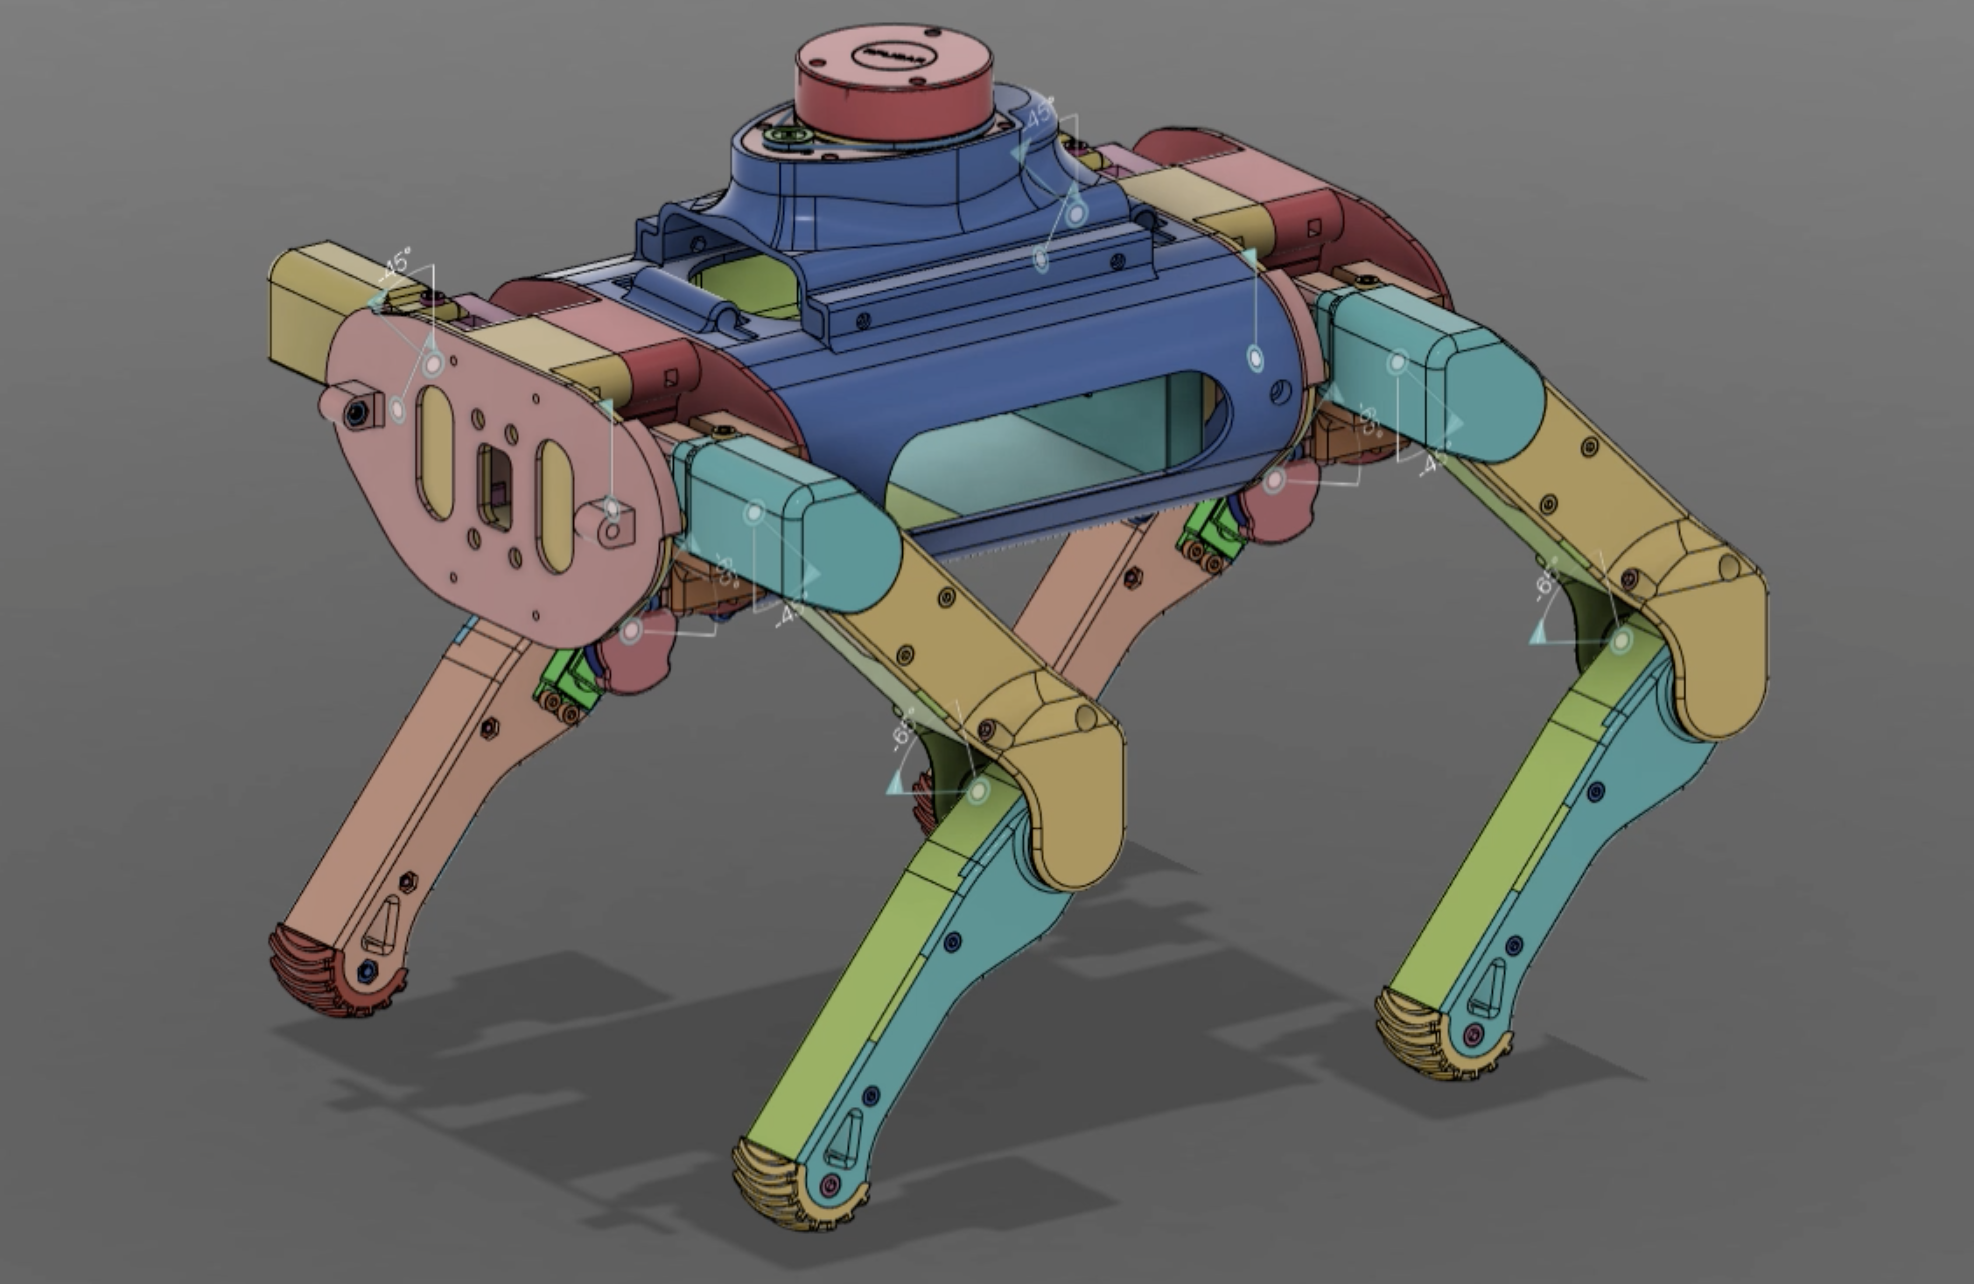
\includegraphics[width=0.5\textwidth]{orbv2F360}
\end{center}


% Processes
\newpage
\chapter{Processes}

% Inverse kinematics
\section{Inverse Kinematics}

\emph{Inverse Kinematics}, abbreviated as \emph{IK}, is a powerful method of control, with which the control problem of positioning the endpoint of a multiple DoF (Degree of Freedom) system can be solved. Here, the endpoint of the multiple DoF system is specified, and the control inputs for the system to achieve the endpoint are computed by the inverse kinematics algorithm.

This find wide application in systems like robotic arms, where the positioning of the arm endpoint can be specified, and joint angles can be computed for positioning the endpoint at the desired location. Similarly, it can be applied to the quadruped leg to compute the leg joint angles from a specified leg endpoint position.

In our quadruped robot, it is used to solve for the three joint angles in each of the four legs, making up a 12 DoF system. Here, we use a [\emph{Hip, Shoulder, Elbow}] nomenclature, which, we admit, is not anatomically accurate. For us, however, it seemed intuitive to think of it in such a way, and thus will continue to use it through the derivation below. The angles are, namely:

\begin{center}
    \(\theta_0 : \) hip joint angle\\
    \(\theta_1 : \) shoulder joint angle\\
    \(\theta_2 : \) elbow joint angle\\
\end{center}

% Insert leg diagrams/figures here
\begin{figure}
    \begin{multicols}{2}
        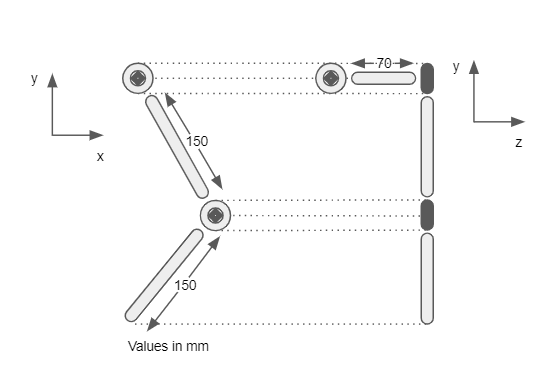
\includegraphics[width=0.5\textwidth]{legFrontSideViewIK}
        \caption{\small Leg views from front, side}
        \label{fig:legViewsIK}
        
        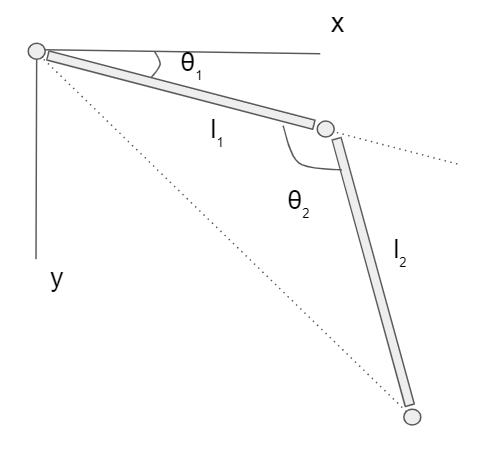
\includegraphics[width=0.3685\textwidth]{legSideViewAnglesIK}
        \caption{\small Annotated side view}
        \label{fig:sideViewAnnIK}
    \end{multicols}     
\end{figure}

Here, we derived our own inverse kinematics algorithm using trigonometric principles, a summary of which is given below.

The notations used in the figures are given below:

\begin{flushleft}
\(x = \) position of the leg endpoint along the x axis\\
\(y = \) position of the leg endpoint along the y axis\\
\(z = \) position of the leg endpoint along the z axis\\
\(l_0 = \) length of leg segment from hip to shoulder\\
\(l_1 = \) length of leg segment from shoulder to elbow\\
\(l_2 = \) length of leg segment from elbow to foot\\
\(l_3 = \) length of front projection from hip to foot\\
\(l_4 = \) length of front projection from shoulder to foot\\
\(r = \) projected leg length from shoulder to foot\\
\(\theta_0 = \) hip joint angle\\
\(\theta_1 = \) shoulder joint angle\\
\(\theta_2 = \) elbow joint angle\\

\end{flushleft}

For the purpose of deriving the relationships of these parameters to the joint angles \(\theta_0\), \(\theta_1\), and \(\theta_2\), we define

\begin{flushleft}
\(\theta_{1 \ effective} = \) effective angle between \(l_3\) and the x axis
\end{flushleft}

% Add annotated front view figure
From Figure \ref{fig:sideViewAnnIK} and Figure, we get \(l_3\) and \(l_4\) as
\[l_3 = \sqrt{y^2 + z^2}\]
\[l_4 = \sqrt{l_3^2 + l_0^2}\]

Now, \(r\) can be found to be
\[r = \sqrt{x^2 + l_4^2}\]

Then, we can compute the hip angle \(\theta_0\) as
\[\theta_0 = \arccos{\left( \frac{z l_0 + y l_4}{l_3^2} \right)}\]

Solving for the knee angle, \(\theta_2\)
\[\cos{\theta_2} = \frac{l_1^2 + l_2^2 - r^2}{2 l_1 l_2}\]

Thus, the knee angle, \(\theta_2\) is given by
\[\theta_2 = \arccos{\left( \frac{l_1^2 + l_2^2 - r^2}{2 l_1 l_2} \right)}\]

Now, we need to solve for the shoulder angle \(\theta_1\). For this,
\[\theta_{1 \ effective} = \arctan{\left( \frac{l_4^2}{x^2} \right)}\]





% Visual odometry
\newpage
\section{Visual Odometry}

Visual Odometry is the process of finding the position and orientation of a robot by analyzing the changes the motion induces on the images of the onboard cameras. It thus intends to find the change in position and rotation of a robot from the \((k)^{th}\) to the \((k+1)^{th}\) image. The result of the visual odometry algorithm is thus a composite translation and rotation matrix, denoted as \(RT\), which can be decomposed to their constituent translation \(T\) and rotation \(R\) matrices, and integrated over several such image pairs to produce an estimate of the state of the robot.

The main advantages of Visual odometry over conventional methods like wheel odometry are :

\begin{itemize}
  \item Not affected by wheel slip in uneven terrain, rainy/snowy weather or other adverse weather conditions.
  \item More accurate trajectory estimates are provided.
\end{itemize}


% Flowchart
\begin{figure}[H]
    \centering
    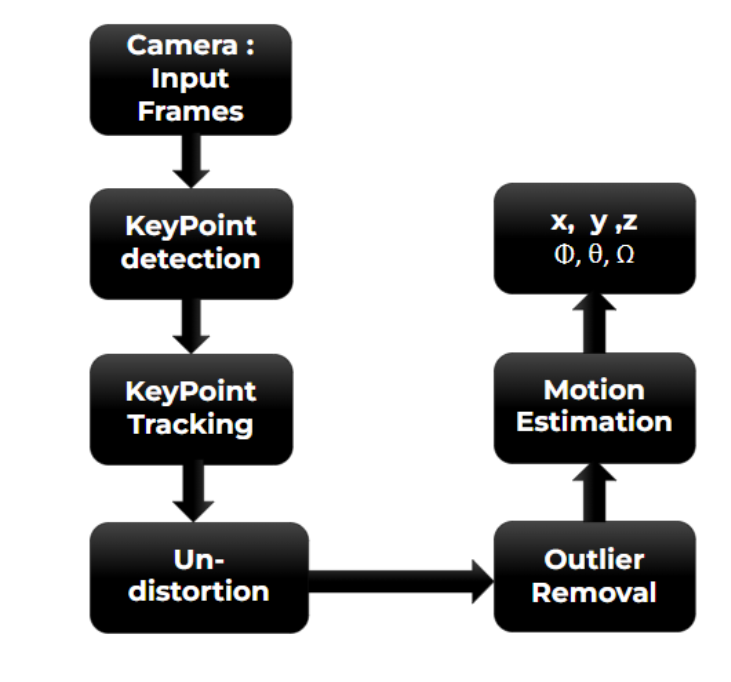
\includegraphics[width=0.9\textwidth]{vo}
    \caption{Flowchart}
    \label{fig:Visual Odometry}
\end{figure}

% Algorithm
\begin{algorithm}[hbt!]
    \caption{Visual odometry algorithm}\label{alg:cap}
    
    \begin{algorithmic}[1]
    
        \Require $img \gets Image\ data\ from\ stereo\ camera$
        \State $Apply\ KeyPoint\ detection\ algorithm\ to\ detection\ $
        \State $Apply\ KeyPoint\ tracking\ algorithm\ $
        \State $Undistortion\ is\ performed\ on\ the\ image\ $
        \State $Perform\ outlier\ removal\ $
        \\
        \Return $Pose$
        
    \end{algorithmic}
\end{algorithm}

\begin{figure}[H]
  \centering
    \begin{multicols}{2}
        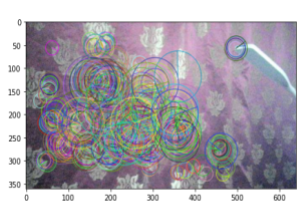
\includegraphics[width=0.5\textwidth]{feature_Detection}
        \caption{Feature Detection}
        \label{fig:Feature Detection}
        
        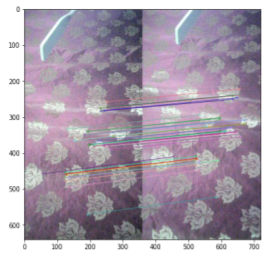
\includegraphics[width=0.5\textwidth]{feature_matching}
        \caption{Feature Matching}
        \label{fig:Feature Matching}
    \end{multicols} 
    
    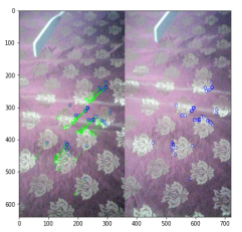
\includegraphics[width=0.5\textwidth]{motion_estimation}
        \caption{Motion Estimation}
        \label{fig:Motion Estimation}
    
\end{figure}

 


% Stair Detection
\newpage
\section{Stair Detection}

% Description
In real-world application, the staircase is a common terrain occurrence. The robot is expected to navigate this terrain autonomously and with ease, thus requiring the implementation of stair detection. The stair detection algorithm takes images of stairs as primary input from the stereo camera setup. With the help of OpenCV fused with Hough Lines algorithm, the raw image data is further processed and refined to produce information about the stair contours, number of steps and step height.\\

% Flowchart
\begin{figure}[H]
    \centering
    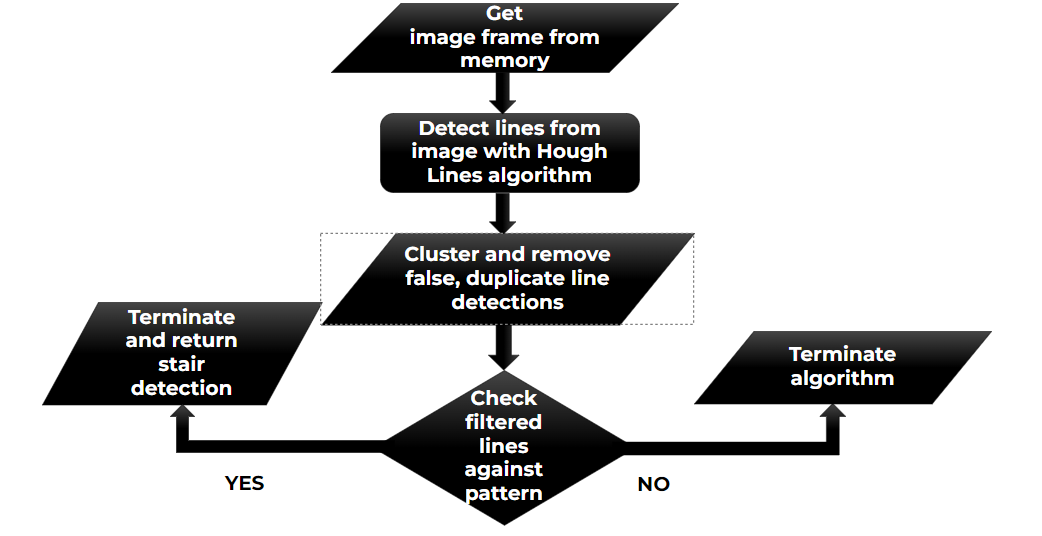
\includegraphics[width=0.9\textwidth]{stairDetect}
    \caption{Flowchart}
    \label{fig:stairDetectionFlowchart}
\end{figure}

% Algorithm
\begin{algorithm}[hbt!]
    \caption{Stair detection algorithm}\label{alg:cap}
    
    \begin{algorithmic}[1]
    
        \Require $img \gets Image\ data\ from\ stereo\ camera$
        \State $Binarize\ img\ to\ reduce\ noise$
        \State $Apply\ Canny\ Edge\ filter\ to\ img$
        \State $Apply\ Hough\ Lines\ filtering\ algorithm\ to\ img$
        \If {$0.1 < \theta < 0.8$}
            \State $\theta =Stair\ side\ angle:Left$
            \State $angleL \gets \theta$
        \ElsIf {$2.4 < \theta < 3$}
            \State $\theta = Stair\ side\ angle:Right$
            \State $angleR \gets \theta$
        \EndIf
        \State $Print\ angleL,\ angleR$
        \If {$91\times \frac{\pi}{180} < \theta <90 \times \frac{\pi}{180}$}
            \State $\theta =Stair\ angle: Vertical $
            \State $angleV \gets \theta$
        \EndIf
        \State $Overlay\ lines\ on\ img$
        \\
        \Return $img$
        
    \end{algorithmic}
\end{algorithm}

\newpage

\begin{figure}[H]
  \centering
    \begin{multicols}{2}
        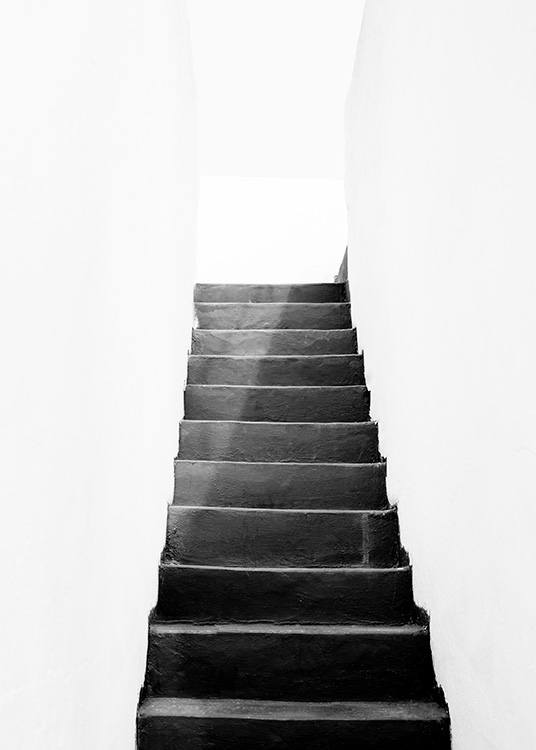
\includegraphics[width=0.3\textwidth]{stairDetectTest_1}
        \caption{Test image}
        \label{fig:testImage}
        
        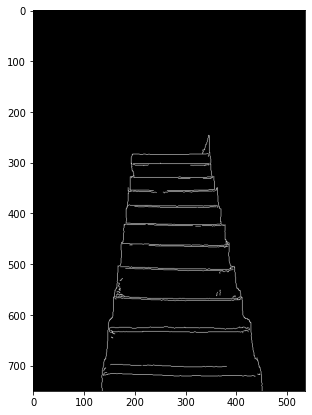
\includegraphics[width=0.33\textwidth]{stairDetectTest_2}
        \caption{Processed image}
        \label{fig:processedImage}
    \end{multicols}     
\end{figure}

\begin{figure}[H]
  \centering
    \begin{multicols}{2}
        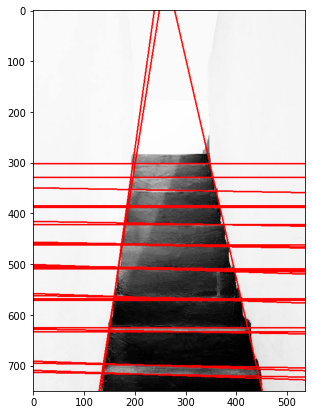
\includegraphics[width=0.3\textwidth]{stairDetectTest_3}
        \caption{Applying Hough Lines algorithm}
        \label{fig:horizontalLinesRaw}
        
        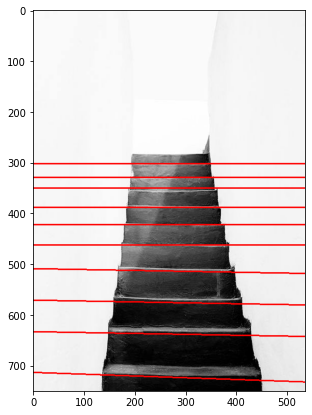
\includegraphics[width=0.3\textwidth]{stairDetectTest_4}
        \caption{Flitered final image}
        \label{fig:horizontalLinesFiltered}
    \end{multicols}     
\end{figure}


%Path Planning
\newpage
\section{Path Planning}

A very cruicial part of autonomous navigation is \emph{path planning}. The robot should be able to successfuly avoid obstacles in its path and choose the shortest path possible to reach its destination to maximize efficiency. For this purpose we need an intelligent and efficient algorithm to enable successful traversal of complex terrain.

In engineering, there are two approaches to solving this problem: mathematical and heuristic approaches. The mathematical approach is more concerned with the solution than with ensuring that the computations are feasible for real-time algorithms. The latter use multiple ways to analyse the overall problem from start to finish. Examples of this apporach include the Euclidean approach to look for geometric patterns and "the look ahead approach". These algorithms, however, don't find the minimum optimal distance. In the heuristic approach, the algorithm uses special knowledge of the problem space. After exploring and studying several algorithms written for path planning, the A* path planning algorithm was chosen for implementing in our robot. The A* algorithm, when used with a proper heuristic for the distance to the destination can generate an optimal path in a graph efficiently. It is the most efficient free-space searching algorithm for path planning and obstacle avoidance, and uses a combination of heuristic searching, and searching based on the shortest path. 

The A* algorithm is classified as a \emph{best-first} algorithm, because each cell in the problem space is evaluated according to the cost of traversal, which is based upon the overall distance of the path. The main benefit of the A* algorithm is its ability to find an optimal solution in a reasonable amount of time, versus the uninformed search of looking for a path. One of the disadvantages of the algorithm is the inability to react to unexpected added or moving obstacles in the testing area. The A* algorithm cannot adjust the list made for creating a path to take or the new bounds not known. The default is there is no path found.

In this algorithm, the whole space is divided into cells or nodes. The starting node and the end node are to be defined initially. The path is found with respect to the distance between these two nodes. The neighbouring nodes of the starting node are first taken into consideration. There are two costs involved in the algorithm, the \(G-cost\) and the \(H-cost\). The \(G-cost\) is the distance between the initial node and the current node, while the heuristic cost or \(H-cost\) is the distance between the current node and the final node, which is an assumption based on distance formulas like the manhattan distance that we have used here. An overall cost called the \(F-cost\) is found for the distance evaluation.

The equation is given below.

\[F-cost = G-cost + H-cost\]

An open list keeps track of the nodes that need to be explored and begins with the start node. This open list, often a \emph{priority queue} data structure is used to keep track of all upcoming nodes. When a path runs out of scope or is not possible to traverse any longer, another nearest neighbour node is taken from the open list.

\[Open = \{(F-cost, \ Node1),(F-cost2, \ Node2), (F-cost2, \ Node2) .... \}\]

This open list is continually updated during the operation of the algorithm.

\newpage
\begin{figure}
    \centering
    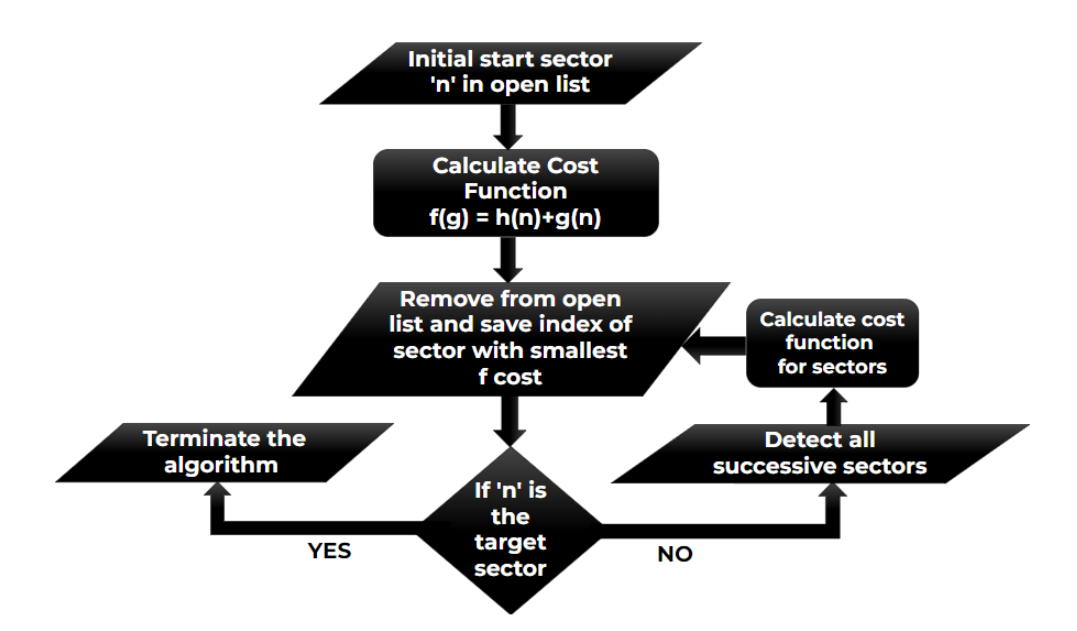
\includegraphics[width=1\textwidth]{Astar}
    \caption{Flowchart}
    \label{fig:pathPlanningFlowchart}
\end{figure}

\vspace{2cm}
\begin{algorithm}[hbt!]
    \caption{A* Path Planning}
    \label{alg:AStarAlgorithm}
    
    \begin{algorithmic}[1]
    
        \Require $ogrid \gets Occupancy \ grid \ data \ from \ RPLiDAR$
        \State $Define \ the \ start \ and \ end\ nodes$
        \State $First \ consider \ unoccupied \ neighbouring \ nodes \ of \ start \ node$
        \State $Evaluate \ G-cost \ and \ H-cost$
        \State $Add \ node \ with \ lowest \ F-cost \ to \ open \ set$
        \State $Consider \ neighboring \ nodes \ with \ lowest \ F-cost \ and \ repeat \ from \ step \ 3 $
        \State $Terminate \ the \ algorithm \ once \ H-cost \ is \ 0 $
        \State $Trace \ back \ last \ nodes\ to \ find \ optimum \ path$
        
    \end{algorithmic}
\end{algorithm}

For example, consider the graph shown in Figure \ref{fig:weightedGraph} with nodes A, B, C and D interconnected with weighted edges, i.e., multiple distance values are associated with the graph.

\begin{figure}[H]
    \centering
    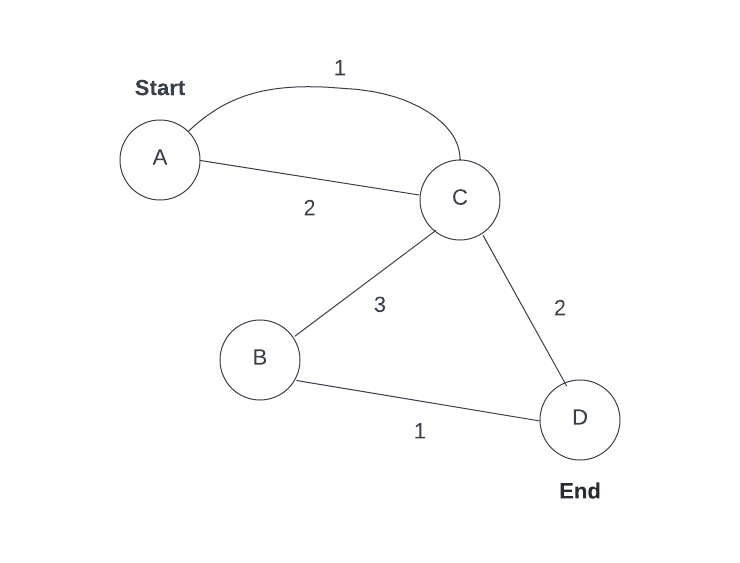
\includegraphics[width=0.45\textwidth]{nodesPath}
    \caption{Weighted graph with nodes A, B, C and D}
    \label{fig:weightedGraph}
\end{figure}

Here the Start node is A and the End node is D. The distance assciated with multiple paths are shown in figure. ie There are 2 ways from A to C, with distance values 1 and 2. The lowest weighted edge is chosen between these two. In this case, the shortest distance between them is 1 and that path is chosen. Thereafter reaching C the G-cost becomes 1 and so on. In the implementation these nodes are considered as the cells of the occupancy grid and the weights for the edges would be set to default as 1, because all the adjacent cells are in equal distances essentially. i.e. If the robot has to cross 2 cells to reach the destination, the distance or the cost would be 2. The intention of the algorithm would be to find the optimum path to reach the destination, here the optimum F-cost would 3 when the path A-C-D is traversed.

To start off with the algorithm we have to insert the start node, along with the F-cost ( initially 0), into the open set, represented by a priority queue. 

\[Open = \{(F-cost, \ Node)\} = \{(0, \ A)\}\]

The inital Costs of the respective nodes are represented in the table.Since we dont consider the start node as a neighbouring node all the values are set defuult to 0. while the other nodes B, C and D have a possibility of being considered as the Neighbouring node and thus the values are set as default to $\infty$. 

\begin{table}[H]
\centering
    \begin{tabular}{ |c|c|c|c| } 
    \hline
    Nodes & F-cost & G-cost & H-cost \\
    \hline 
    A & 0 & 0 & 0\\ 
    B & $\infty$ & $\infty$ & $\infty$\\ 
    C & $\infty$ & $\infty$ & $\infty$\\ 
    D & $\infty$ & $\infty$ & $\infty$\\
    \hline
    \end{tabular}
    \caption{Nodes and their costs}
    \label{table:nodeCost0}
\end{table}

Now the first neighbouring node C is considered and the lowes G cost available to it is 1 and using the manhattan distance formula the h-cost is assumed to be 1 although the value might be incorrect. Then the overall f cost is 2. and the last node we came from is A. 

\begin{table}[H]
\centering
    \begin{tabular}{ |c|c|c|c|c| } 
    \hline
    Nodes & F-cost & G-cost & H-cost & Last Node \\
    \hline 
    A & 0 & 0 & 0 &\\ 
    B & $\infty$ & $\infty$ & $\infty$ &\\ 
    C & 2 & 1 & 1 & A\\ 
    D & $\infty$ & $\infty$ & $\infty$ &\\
    \hline
    \end{tabular}
    \caption{Nodes and their costs}
    \label{table:nodeCost1}
\end{table}

Now this node aloong with its F-cost is added to the open set of neighbouring nodes.

\[Open = \{(2, \ C)\}\]

In the open set there is only one node so there is no comparisson to make with respect to the shortest F-cost.Now we consider the Node C and its neighbours, D and B. In the case of B the G-cost is 4 and H-cost is assumed, while in the case of D, the G-cost is 3. 
    The table is updated as shown below

\begin{table}[H]
\centering
    \begin{tabular}{ |c|c|c|c|c| } 
    \hline
    Nodes & F-cost & G-cost & H-cost & Last Node \\
    \hline     
    A & 0 & 0 & 0 &\\ 
    B & 6 & 4 & 2 & C\\ 
    C & 2 & 1 & 1 & A\\ 
    D & 3 & 3 & 0 & C\\
    \hline
    \end{tabular}
    \caption{Nodes and their costs}
    \label{table:nodeCost2}
\end{table}

Therefore the node with the lower F-cost, D, is added to the open set and the node B is ignored.The value of H-cost is 0 for node D, since it is the end node.

\[Open = \{(2, \ C)\}, \{(3, \ D)\}\]

While comparing the F-costs of the nodes in the open set, we find the End node and its taken out of the open set to complete the algorithm.

Now all we have to do is backtrack all the last nodes. i.e. D from C, C from A, and thus we get the optimum path, A-C-D.

For the purpose of visualization additional python packages were used. \emph{PyGame} is a 2-D graphics module for python, which is easy to use and was used to implement the visualization tool effectively. 

The occupancy grid is generated from the data produced by the RPLiDAR unit. For purposes of visualization, we set the Start Node (in Orange), End node (in Turquoise), and Occupied Nodes (in Black), with the unoccupied Nodes represented in white. The reconstructed path is represented in purple, and is the optimum path for the robot to reach its destination.

The input and output images of the Pygame window are given in Figure \ref{fig:occupancyGrid} and Figure \ref{fig:reconstructedPath}.\\

\begin{figure}[H]
    \begin{multicols}{2}
    \centering
        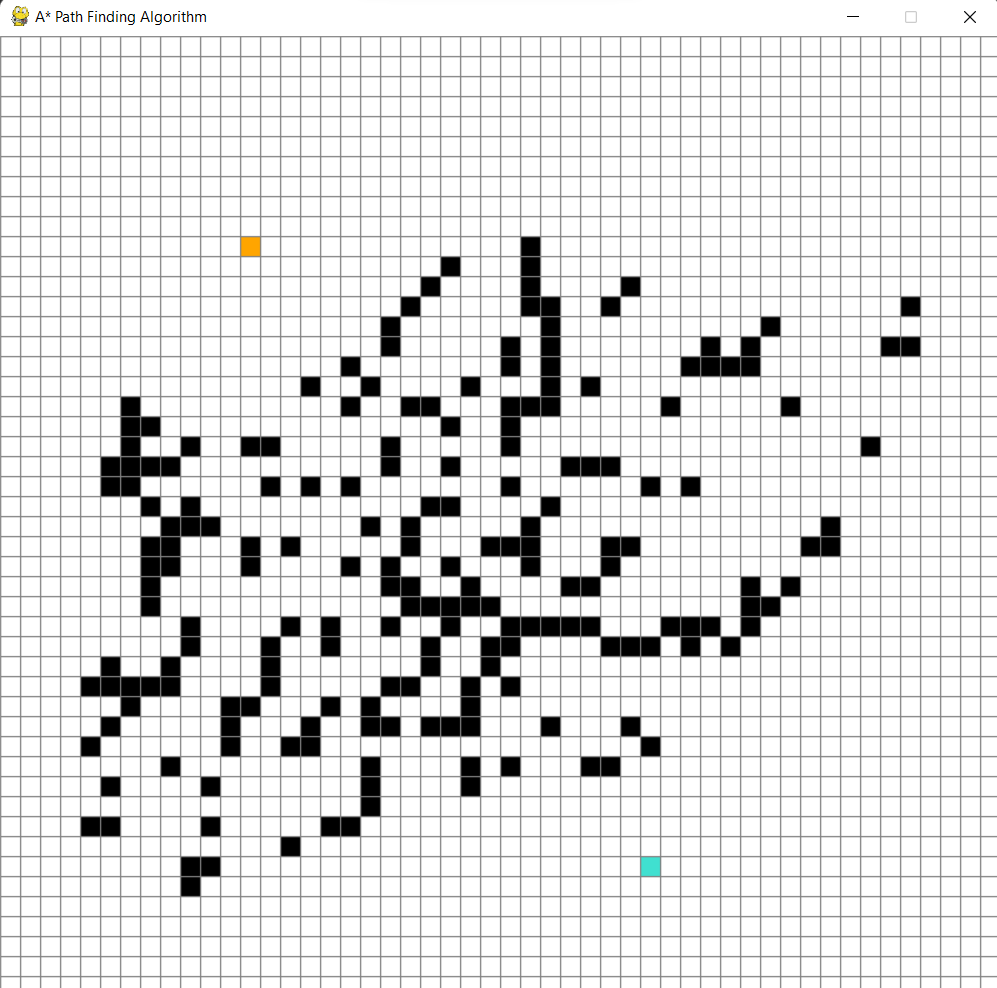
\includegraphics[width=0.35\textwidth]{Astarinput}\\
        \caption{Occupancy grid}
        \label{fig:occupancyGrid}

        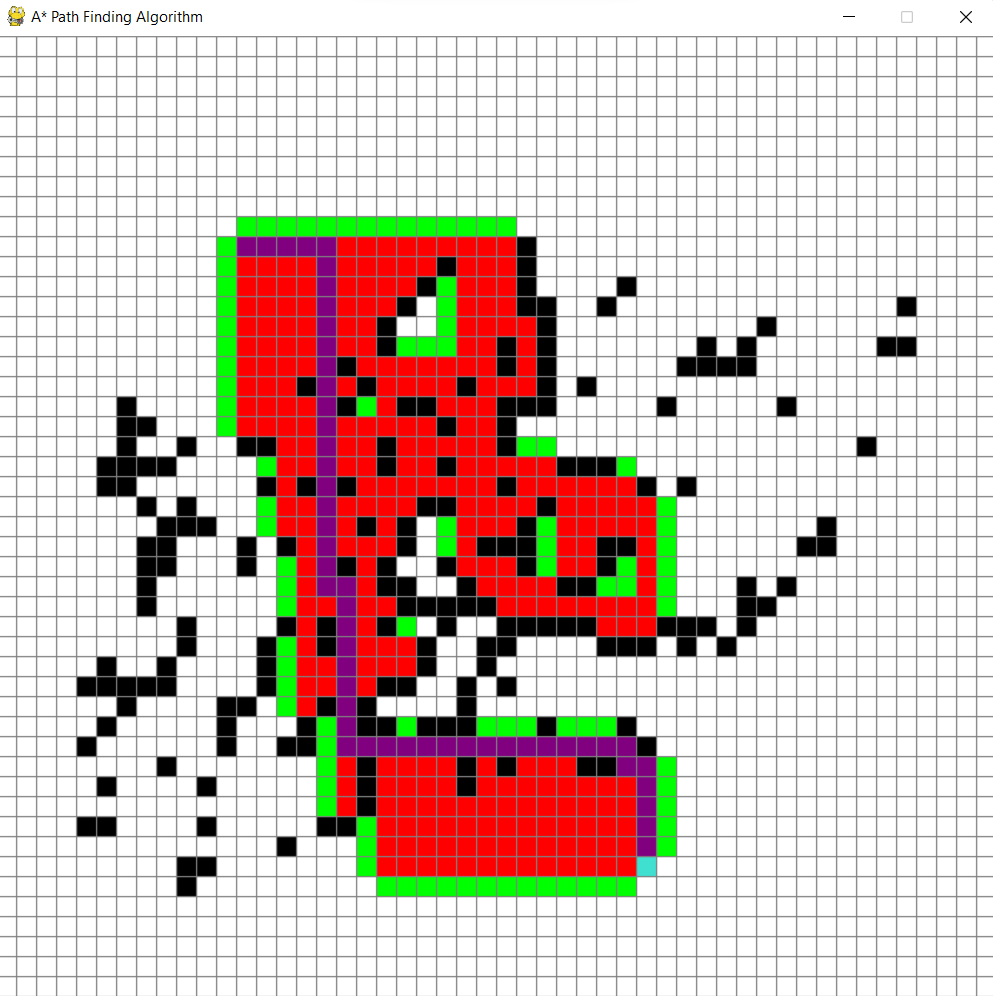
\includegraphics[width=0.35\textwidth]{Astaroutput}\\
        \caption{Reconstructed Path}
        \label{fig:reconstructedPath}
    \end{multicols}
\end{figure}




\end{document}